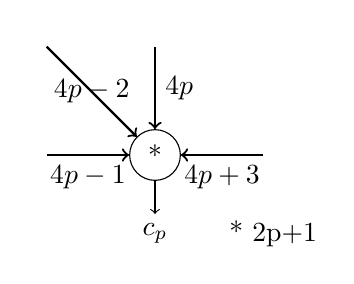
\begin{tikzpicture}[scale=0.5]

    \tikzset{nodestyle/.style={draw,shape=circle}}
    \node (p2) at ( 3, 0) {};
    \node (p33) at (9,-2) {* 2p+1};
    \node[nodestyle] (p3) at ( 6, 0) {*};
    \node (p4) at ( 9, 0) {};

    \node (p8) at ( 3, 3) {};
    \node (p9) at ( 6, 3) {};

    \begin{scope}[every path/.style={->,thick}]
        \draw (p2) -- (p3)node[midway,below]{$4p-1$}; 
        \draw (p4) -- (p3)node[midway,below]{$4p+3$};

        \draw (p9) -- (p3)node[midway,right]{$4p$};
        \draw (p8) -- (p3)node[midway]{$4p-2$};

    \end{scope} 
    \node (c2) at ( 6, -2) {$c_p$};

        \draw[->] (p3) -- (c2);
\end{tikzpicture}
